\subsection{Real Data}
We now present the results of running the algorithm on several real life datasets. Two of the merchants had moderate-sized relation graphs with about $10^5$ vertices and $10^6$ relations (candidate recommendation edges);  the remaining merchants (3, 4 and 5) have on the order of $10^6$ products and $10^7$ relations between them. The sizes of the true optimal solutions for these recommendation problems were unknown to us, and we estimated this quantity by taking the minimum of $|L|c/a$ and the number of vertices in $R$ of degree at least $a$. Note that this is an upper bound on OPT, and that the true optimal value is very likely lower than this estimate. Figures~\ref{fig:real_sampling},~\ref{fig:real_greedy} and~\ref{fig:real_partition} plot the average of the optimality percentage of the sampling, greedy and partition algorithms across all the merchants respectively. Note that we could only run the partition algorithm for the first two merchants due to memory constraints. \vs

\begin{figure}[t]
\centering
\begin{minipage}[h]{0.48\textwidth}
\centering
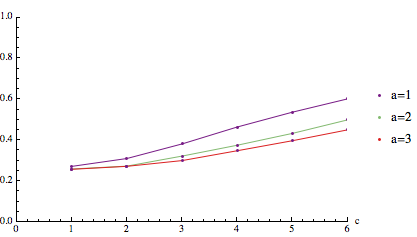
\includegraphics[width=0.8\textwidth]{images/real_sampling.png}
\caption{Sampling algorithm for real merchants}\label{fig:real_sampling}
\end{minipage}
\hspace{0cm}
\begin{minipage}[h]{0.48\textwidth}
\centering
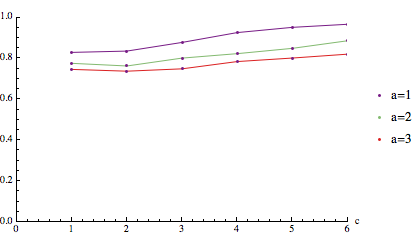
\includegraphics[width=0.8\textwidth]{images/real_greedy.png}
\caption{Greedy algorithm for real merchants}\label{fig:real_greedy}
\end{minipage}
\hspace{0cm}
\centering
\begin{minipage}[h]{0.48\textwidth}
\centering
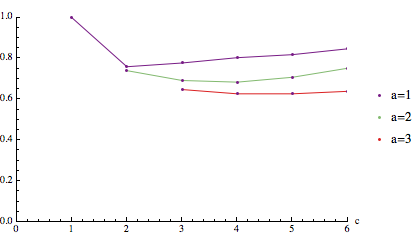
\includegraphics[width=0.8\textwidth]{images/real_partition.png}
\caption{Partition algorithm for real merchants}\label{fig:real_partition}
\end{minipage}
\vspace{-0.2in}
\end{figure} \vs

From these results, we can see that that greedy performs exceptionally well when $c$ gets even moderately large.
For the realistic value of $c=6$, the greedy algorithm produced a solution that was 85\% optimal for all the
merchants we tested. For several of the merchants, its results were almost optimal starting from $a=2$. \vs

The partition method is also promising, especially when the $a$ value that is targeted is low. Indeed, when $a=1$ or $a=2$,
it's performance is comparable to that of greedy, though it lags behind what the simulated runs would suggest.
In some of the low-$a$ instances, the partition algorithm still beats the greedy algorithm. However, as $a$ gets larger,
the partition algorithm gets worse faster than the other algorithms since each matchings it finds is not ``informed" or guided by other matchings it constructs in other disjoint parts of the graph. While this decomposition of edges gives us algorithmic efficiency, it also results in a rapid loss of quality. \vs

The sampling algorithm performs mostly well in real life data, but and particularly so when $c$ gets large. It is typically worse than greedy, but unlike the partition algorithm, it's performance improves dramatically as $c$ gets larger, and it's performance does not get worse as quickly when $a$ gets larger. Therefore, as $c$ gets larger, it becomes a viable alternative to greedy mainly in cases where the $O(|L|)$ memory cost of the greedy algorithm is too prohibitive. It is therefore impractical to use on all but the largest of data sets. 
